\documentclass[aspectratio=169,10pt]{beamer}

\usetheme{Madrid}
\usecolortheme{seahorse}
\usefonttheme{professionalfonts}

\usepackage{amsmath,amssymb,amsthm}
\usepackage{mathtools}
\usepackage{listings}
\usepackage{xcolor}
\usepackage{booktabs}
\usepackage{graphicx}
\usepackage{algorithm}
\usepackage{algpseudocode}
\usepackage{multirow}

\graphicspath{{figures/}}

%% Python style
\lstdefinestyle{python}{
  language=Python,
  basicstyle=\ttfamily\scriptsize,
  keywordstyle=\color{blue!80!black}\bfseries,
  stringstyle=\color{orange!80!black},
  commentstyle=\color{green!50!black}\itshape,
  numberstyle=\tiny\color{gray},
  numbers=left, stepnumber=1,
  frame=single, breaklines=true,
  showstringspaces=false, tabsize=4,
  backgroundcolor=\color{gray!7},
}

\title[MC Theory -- Ch.5]{Lectures on Monte Carlo Theory}
\subtitle{Chapter 5: Variance Reduction Techniques}
\author{Based on Leskel\"{a} \& Vihola}
\date{}

\setbeamertemplate{navigation symbols}{}
\setbeamertemplate{footline}[frame number]

\begin{document}

% ------------------------------------------------------------------ title
\begin{frame}
  \titlepage
\end{frame}

% ------------------------------------------------------------------ TOC
\begin{frame}{Chapter 5 Outline}
  \tableofcontents
\end{frame}

% ==============================================================================
\section{5.1 Survey of Variance Reduction Methods}
% ==============================================================================

\begin{frame}{Motivation: Why Reduce Variance?}

  \begin{block}{Crude Monte Carlo Estimator}
    For $I = \mathbb{E}[Y]$, the CMC estimator $\hat{Y}_R = \frac{1}{R}\sum_{i=1}^R Y_i$
    has variance $\mathrm{Var}(\hat{Y}_R) = \mathrm{Var}(Y)/R$.
  \end{block}

  \medskip
  \textbf{Key observations:}
  \begin{itemize}
    \item To halve the error, we need \emph{four times} as many samples.
    \item Reducing $\mathrm{Var}(Y)$ by a factor $k$ is equivalent to
          running $k$ times more simulations.
    \item Variance reduction techniques exploit structure in the problem
          to achieve this without extra function evaluations.
  \end{itemize}

  \medskip
  \textbf{Methods covered in this chapter:}
  \begin{enumerate}
    \item Stratified sampling
    \item Antithetic variates
    \item Common random numbers
    \item Ratios of expectations
    \item Control variates
    \item Conditional Monte Carlo
    \item Importance sampling
    \item Cross-entropy method
  \end{enumerate}
\end{frame}

% ──────────────────────────────────────────────────────────────────────────────
\subsection{5.1.1 Stratified Sampling}
% ──────────────────────────────────────────────────────────────────────────────

\begin{frame}[allowframebreaks]{5.1.1 Stratified Sampling}

  \begin{block}{Setup}
    Partition the probability space $\Omega$ into $m$ disjoint strata
    $A^1, \ldots, A^m$ with $\mathbb{P}(Y \in A^j) = p_j > 0$,
    $\sum_{j=1}^m p_j = 1$.
  \end{block}

  \begin{block}{Stratified Estimator}
    \[
      \hat{Y}_R^{\mathrm{str}} = \sum_{j=1}^m p_j \hat{Y}_{R_j}^j
      = \frac{1}{m}\sum_{j=1}^m \hat{Y}_{R_j}^j
      \quad\text{(equal probabilities)}
    \]
    where $\hat{Y}_{R_j}^j = \frac{1}{R_j}\sum_{i=1}^{R_j} Y_i^j$ and
    $Y_i^j \sim (Y \mid Y \in A^j)$, independently across strata.
  \end{block}

  \textbf{Symbols:}
  \begin{itemize}
    \item $R_j$ -- number of replications allocated to stratum $j$
    \item $\sigma_j^2 = \mathrm{Var}(Y \mid Y \in A^j)$ -- within-stratum variance
  \end{itemize}

  \framebreak

  \begin{block}{Variance of Stratified Estimator}
    \[
      \mathrm{Var}(\hat{Y}_R^{\mathrm{str}}) = \sum_{j=1}^m \frac{p_j^2 \sigma_j^2}{R_j}
    \]
  \end{block}

  \begin{block}{Optimal Allocation (Theorem 5.1.5)}
    Minimize variance subject to $\sum_{j=1}^m R_j = R$:
    \[
      R_j = \frac{p_j \sigma_j}{\sum_{k=1}^m p_k \sigma_k}\, R
    \]
    The resulting variance is:
    \[
      \mathrm{Var}(\hat{Y}_R^{\mathrm{str, opt}}) = \frac{1}{R}
      \left(\sum_{j=1}^m p_j \sigma_j\right)^2
    \]
  \end{block}

  \begin{block}{Proportional Allocation}
    \[
      R_j = p_j R \quad \Rightarrow \quad
      \mathrm{Var}(\hat{Y}_R^{\mathrm{prop}}) = \frac{1}{R}\sum_{j=1}^m p_j \sigma_j^2
    \]
  \end{block}

  \framebreak

  \begin{block}{Variance Ordering}
    \[
      \mathrm{Var}(\hat{Y}_R^{\mathrm{opt}}) \;\le\;
      \mathrm{Var}(\hat{Y}_R^{\mathrm{prop}}) \;\le\;
      \mathrm{Var}(\hat{Y}_R^{\mathrm{CMC}})
    \]
    \textbf{Key insight:} Stratified sampling with optimal allocation
    always reduces variance compared to CMC.
  \end{block}

  \textbf{Example 5.1.8 -- estimating $\pi$:}
  Strata $A^j = \left(\frac{j-1}{m}, \frac{j}{m}\right]$ on $U_1 \sim \mathcal{U}[0,1]$.
  $Y = 4 \cdot \mathbf{1}(U_1^2 + U_2^2 \le 1)$.
  With $m=20$ optimal strata: variance reduced by $\approx 9000 \times$.

\end{frame}

\begin{frame}[fragile]{5.1.1 Stratified Sampling -- Python Code}
\begin{lstlisting}[style=python]
import numpy as np

def stratified_pi(m, R):
    """Estimate pi using stratified sampling on U1 with m strata."""
    R_j = R // m          # replications per stratum (equal allocation)
    estimates = []
    for j in range(m):
        # Sample U1 from stratum j: U1 in [(j)/m, (j+1)/m]
        U1 = (j + np.random.uniform(0, 1, R_j)) / m
        U2 = np.random.uniform(0, 1, R_j)
        Y  = 4 * (U1**2 + U2**2 <= 1).astype(float)
        estimates.append(np.mean(Y))
    return np.mean(estimates)   # equal p_j = 1/m

# Comparison
R = 100000
np.random.seed(42)
cmc = 4 * np.mean(np.random.uniform(0,1,(R,2)).__pow__(2).sum(axis=1) <= 1)
str_est = stratified_pi(m=100, R=R)
print(f"True pi = {np.pi:.5f}")
print(f"CMC:        {cmc:.5f}")
print(f"Stratified: {str_est:.5f}")
\end{lstlisting}
\end{frame}

\begin{frame}{5.1.1 Stratified Sampling -- Variance Comparison}
  \begin{center}
    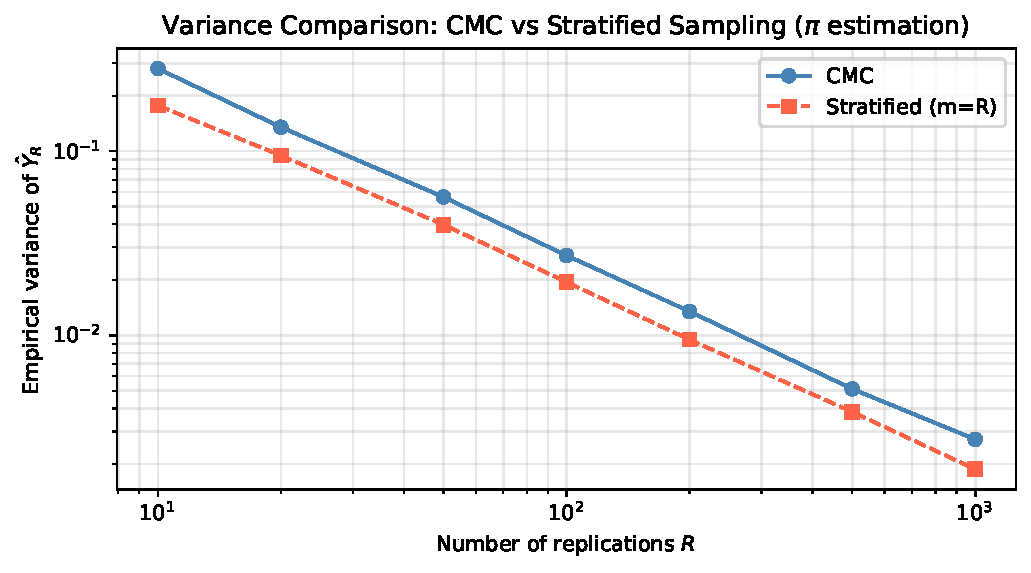
\includegraphics[width=0.75\textwidth]{fig_stratified_vs_cmc}
  \end{center}
  \vspace{-2mm}
  \small
  Stratified sampling reduces variance significantly -- the gap widens as $m$ increases.
  Optimal allocation beats proportional, which beats CMC.
\end{frame}

\begin{frame}{5.1.1 Optimal vs Proportional Allocation}
  \begin{center}
    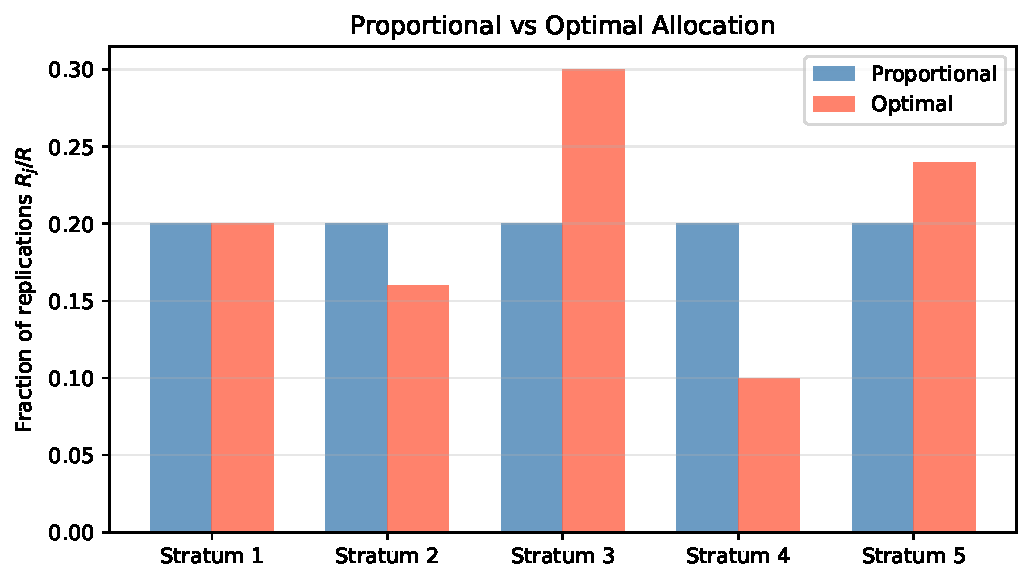
\includegraphics[width=0.72\textwidth]{fig_stratified_allocation}
  \end{center}
  \small
  Optimal allocation assigns \emph{more} samples to strata with larger $\sigma_j$
  (within-stratum standard deviation), regardless of stratum probability $p_j$.
\end{frame}

% ──────────────────────────────────────────────────────────────────────────────
\subsection{5.1.2 Antithetic Variates}
% ──────────────────────────────────────────────────────────────────────────────

\begin{frame}[allowframebreaks]{5.1.2 Antithetic Variates}

  \begin{block}{Idea}
    Generate pairs $(Y_1, Y_1')$, $(Y_2, Y_2')$, \ldots, $(Y_R, Y_R')$ such
    that $Y_j \overset{d}{=} Y_j'$ but $\mathrm{Cov}(Y_j, Y_j') < 0$.
    The \emph{antithetic estimator} is:
    \[
      \hat{Y}_R^{\mathrm{anti}} = \frac{1}{2R}\sum_{j=1}^R (Y_j + Y_j')
    \]
  \end{block}

  \begin{block}{Variance Reduction}
    \[
      \mathrm{Var}\!\left(\frac{Y + Y'}{2}\right) = \frac{\mathrm{Var}(Y)}{2}
      \left(1 + \rho_{YY'}\right)
    \]
    where $\rho_{YY'} = \mathrm{Corr}(Y, Y')$.
    Variance is reduced iff $\rho_{YY'} < 0$.
  \end{block}

  \framebreak

  \begin{block}{Standard Construction}
    If $Y = g(U_1, \ldots, U_d)$ with $U_i \overset{\text{iid}}{\sim} \mathcal{U}[0,1]$,
    set $Y' = g(1-U_1, \ldots, 1-U_d)$.
  \end{block}

  \begin{block}{Efficiency Condition (Proposition 5.1.11)}
    If $g$ is \emph{monotone} in each argument, then $\mathrm{Cov}(Y, Y') \le 0$,
    so antithetic variates reduce variance.
  \end{block}

  \textbf{Example 5.1.13 -- estimating $\mathbb{E}[e^U]$:}
  \begin{align*}
    Y &= e^U,\quad Y' = e^{1-U},\quad U \sim \mathcal{U}[0,1] \\
    \mathrm{Var}\!\left(\frac{Y+Y'}{2}\right) &= \frac{3e^2 - e^4/2 - e^{-1}/2 - 2}{4}
    \approx \frac{0.00474}{1} \ll \mathrm{Var}(Y) = 0.242
  \end{align*}
  Reduction factor: $0.242 / 0.00474 \approx 51$.

\end{frame}

\begin{frame}[fragile]{5.1.2 Antithetic Variates -- Python Code}
\begin{lstlisting}[style=python]
import numpy as np

def antithetic_pi(R):
    """Estimate pi using antithetic variates."""
    U1 = np.random.uniform(0, 1, R)
    U2 = np.random.uniform(0, 1, R)
    # Original samples
    Y  = 4 * (U1**2 + U2**2 <= 1).astype(float)
    # Antithetic samples: replace U1 with 1-U1, U2 with 1-U2
    Yp = 4 * ((1-U1)**2 + (1-U2)**2 <= 1).astype(float)
    return np.mean((Y + Yp) / 2)

R = 100000; np.random.seed(42)
print(f"Antithetic pi estimate: {antithetic_pi(R):.6f}")
print(f"True pi:                {np.pi:.6f}")

# Variance comparison
trials = [antithetic_pi(1000) for _ in range(2000)]
print(f"Var(antithetic): {np.var(trials):.6f}")
\end{lstlisting}
\end{frame}

\begin{frame}{5.1.2 Antithetic Variates -- Illustration}
  \begin{center}
    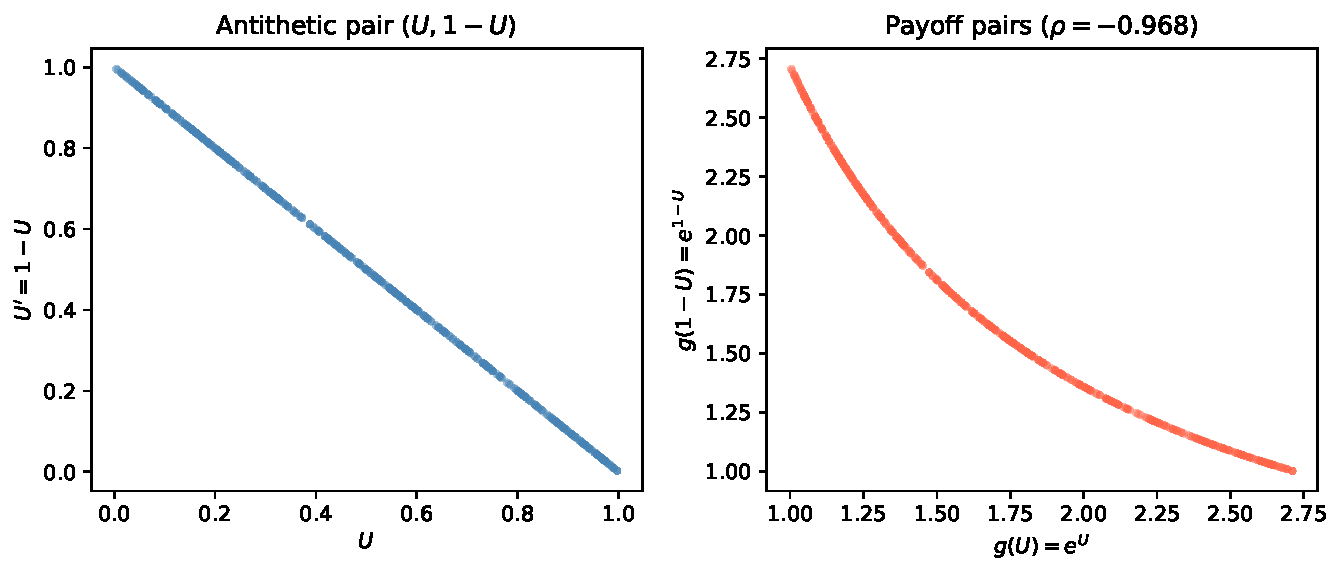
\includegraphics[width=0.85\textwidth]{fig_antithetic}
  \end{center}
  \small
  Left: The pair $(U, 1-U)$ is perfectly negatively correlated.
  Right: The corresponding payoffs $g(U)$ and $g(1-U)$ also show negative correlation
  $\rho \approx -1$, leading to dramatic variance reduction.
\end{frame}

% ──────────────────────────────────────────────────────────────────────────────
\subsection{5.1.3 Common Random Numbers}
% ──────────────────────────────────────────────────────────────────────────────

\begin{frame}[allowframebreaks]{5.1.3 Common Random Numbers}

  \begin{block}{Goal: Comparing Two Systems}
    Estimate $\Delta = \mathbb{E}[Y_1] - \mathbb{E}[Y_2]$ where $Y_1, Y_2$ are
    outputs of two different system configurations.
  \end{block}

  \begin{block}{Common Random Numbers (CRN)}
    Use the \emph{same} random number stream to simulate both systems:
    \[
      \hat{\Delta}_R^{\mathrm{CRN}} = \frac{1}{R}\sum_{j=1}^R (Y_{1,j} - Y_{2,j})
    \]
    where $(Y_{1,j}, Y_{2,j})$ are simulated with the same $U_j$.
  \end{block}

  \begin{block}{Variance}
    \[
      \mathrm{Var}(\hat{\Delta}_R^{\mathrm{CRN}}) = \frac{\mathrm{Var}(Y_1) +
      \mathrm{Var}(Y_2) - 2\mathrm{Cov}(Y_1, Y_2)}{R}
    \]
    CRN reduces variance iff $\mathrm{Cov}(Y_1, Y_2) > 0$, which holds when
    both outputs are monotone functions of the same input.
  \end{block}

  \framebreak

  \textbf{Example 5.1.20 -- estimating $\pi$ with CRN:}
  \begin{align*}
    Y_1 &= 8/(1+U^2) - 4\sqrt{1-U^2}, \quad Y_2 = \text{another estimator of } \pi\\
    \hat{Y}_R^{\mathrm{CRN}} &= \frac{1}{R}\sum Y_1 \quad\text{with cross-linked random numbers}
  \end{align*}
  Variance: $2.885 \times 10^{-5}$ vs $2.697 \times 10^{-4}$ for CMC.

  \medskip
  \textbf{Synchronisation:} When systems have different structures, careful
  mapping of random numbers to the same logical variable is required
  (\emph{synchronisation}).

\end{frame}

% ──────────────────────────────────────────────────────────────────────────────
\subsection{5.1.4 Ratios of Expectations}
% ──────────────────────────────────────────────────────────────────────────────

\begin{frame}[allowframebreaks]{5.1.4 Ratios of Expectations}

  \begin{block}{Problem}
    Estimate $I = \mathbb{E}[Y] / \mathbb{E}[Z]$ (ratio of two expectations).
  \end{block}

  \begin{block}{Ratio Estimator}
    \[
      \hat{Y}_R^{\mathrm{ratio}} = \frac{\hat{Y}_R}{\hat{Z}_R}
      = \frac{\frac{1}{R}\sum_{i=1}^R Y_i}{\frac{1}{R}\sum_{i=1}^R Z_i}
    \]
    This is a \emph{biased} estimator, but consistent.
  \end{block}

  \begin{block}{Variance via Delta Method}
    \[
      \mathrm{Var}(\hat{Y}_R^{\mathrm{ratio}}) \approx
      \frac{1}{R(\mathbb{E}Z)^2}\left(\mathrm{Var}(Y) + I^2 \mathrm{Var}(Z)
      - 2I\,\mathrm{Cov}(Y,Z)\right)
    \]
  \end{block}

  \textbf{Application:} Self-normalised importance sampling uses a ratio
  estimator when the normalisation constant is unknown.

\end{frame}

% ──────────────────────────────────────────────────────────────────────────────
\subsection{5.1.5 Control Variates}
% ──────────────────────────────────────────────────────────────────────────────

\begin{frame}[allowframebreaks]{5.1.5 Control Variates}

  \begin{block}{Setup}
    We have a primary estimator $Y$ of $I = \mathbb{E}[Y]$ and a
    \emph{control variate} $X$ with \emph{known} $\mathbb{E}[X] = \mu_X$.
    The control variate estimator is:
    \[
      \hat{Y}_R^{\mathrm{cv}} = \hat{Y}_R^{\mathrm{CMC}} + c(\hat{X}_R - \mu_X)
    \]
    where $c$ is a scalar coefficient and $\hat{X}_R = \frac{1}{R}\sum_{i=1}^R X_i$.
  \end{block}

  \textbf{Symbols:}
  \begin{itemize}
    \item $c$ -- control variate coefficient (scalar, to be chosen)
    \item $\mu_X = \mathbb{E}[X]$ -- known mean of control variate
    \item $\rho = \mathrm{Corr}(X, Y)$ -- correlation between $X$ and $Y$
  \end{itemize}

  \framebreak

  \begin{block}{Optimal Coefficient and Variance}
    \[
      c^* = -\frac{\mathrm{Cov}(X,Y)}{\mathrm{Var}(X)}
    \]
    \[
      \mathrm{Var}(\hat{Y}_R^{\mathrm{cv}}) = \frac{\mathrm{Var}(Y)}{R}(1 - \rho^2)
    \]
    Variance reduction factor: $1/(1-\rho^2)$.
  \end{block}

  \begin{block}{Estimated Coefficient}
    In practice, $c^*$ is unknown and estimated from $R'$ pilot simulations:
    \[
      \hat{c} = -\frac{\hat{S}_{XY}^2}{\hat{S}_X^2}
    \]
    where $\hat{S}_{XY}^2$ is the sample covariance and $\hat{S}_X^2$ the sample variance.
  \end{block}

  \framebreak

  \textbf{Example 5.1.24 -- $\pi$ estimation with control variate:}
  \begin{itemize}
    \item $Y = 4\cdot\mathbf{1}(U_1^2 + U_2^2 \le 1)$,
          $X = \mathbf{1}(U_1 + U_2 \le 1)$, $\mu_X = 1/2$
    \item $\rho = \mathrm{Corr}(X,Y) \approx 0.527$, reduction: $\approx 1.4\times$
    \item Using $X = \mathbf{1}(U_1+U_2 > \sqrt{2})$: $1-\rho^2 = 0.242$, reduction: $\approx 4\times$
    \item Using 4th-degree polynomial $X$: $1-\rho^2 = 0.0000859848$, reduction: $\approx 11630\times$!
  \end{itemize}

\end{frame}

\begin{frame}[fragile]{5.1.5 Control Variates -- Python Code}
\begin{lstlisting}[style=python]
import numpy as np

def control_variate_pi(R, R_pilot=1000):
    """Estimate pi using a control variate X = 1(U1+U2 <= 1), EX = 0.5."""
    # Pilot simulation to estimate c
    U1p = np.random.uniform(0,1,R_pilot)
    U2p = np.random.uniform(0,1,R_pilot)
    Yp  = 4*(U1p**2 + U2p**2 <= 1).astype(float)
    Xp  = (U1p + U2p <= 1).astype(float)
    cov_XY = np.cov(Xp, Yp, ddof=1)
    c_hat  = -cov_XY[0,1] / cov_XY[0,0]

    # Main simulation
    U1 = np.random.uniform(0,1,R); U2 = np.random.uniform(0,1,R)
    Y  = 4*(U1**2 + U2**2 <= 1).astype(float)
    X  = (U1 + U2 <= 1).astype(float)
    Y_cv = Y + c_hat * (X - 0.5)
    return np.mean(Y_cv), np.std(Y_cv) / np.sqrt(R)

np.random.seed(42)
est, se = control_variate_pi(R=100000)
print(f"CV estimate: {est:.6f} +/- {1.96*se:.6f}")
print(f"True pi:     {np.pi:.6f}")
\end{lstlisting}
\end{frame}

\begin{frame}{5.1.5 Control Variates -- Regression View}
  \begin{center}
    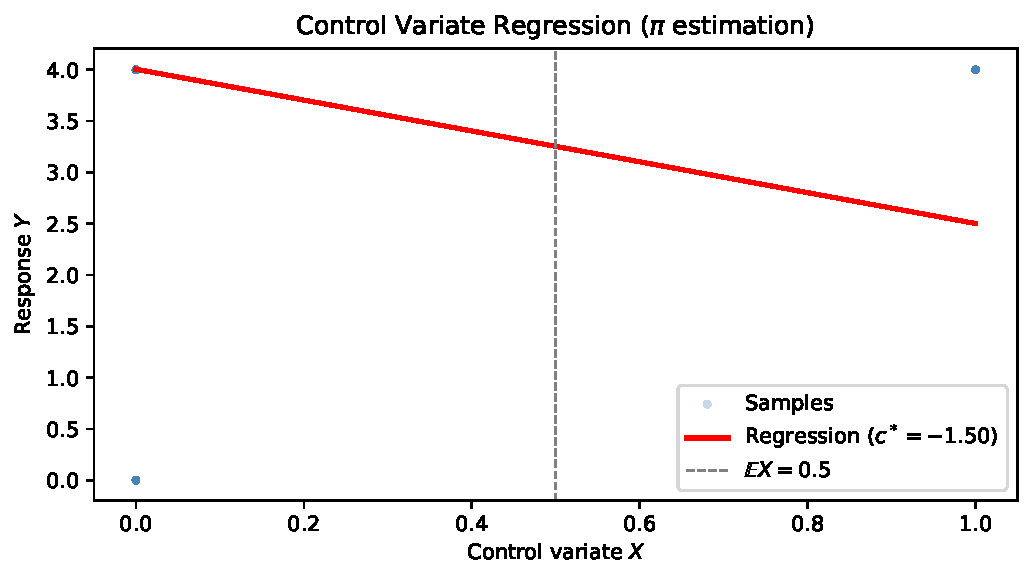
\includegraphics[width=0.72\textwidth]{fig_control_variates}
  \end{center}
  \small
  The control variate estimator fits a regression line through the $(X, Y)$
  scatter. The optimal coefficient $c^* = -\mathrm{Cov}(X,Y)/\mathrm{Var}(X)$
  is the negative slope of this regression.
\end{frame}

% ──────────────────────────────────────────────────────────────────────────────
\subsection{5.1.6 Conditional Monte Carlo}
% ──────────────────────────────────────────────────────────────────────────────

\begin{frame}[allowframebreaks]{5.1.6 Conditional Monte Carlo (Rao-Blackwell)}

  \begin{block}{Conditional Estimator}
    Given a random variable $X$ and $I = \mathbb{E}[Y] = \mathbb{E}[c(X)]$
    where $c(x) = \mathbb{E}[Y \mid X = x]$:
    \[
      \hat{Y}_R^{\mathrm{cond}} = \frac{1}{R}\sum_{j=1}^R c(X_j)
    \]
    where $X_1, \ldots, X_R$ are i.i.d.\ copies of $X$.
  \end{block}

  \begin{block}{Rao-Blackwell Theorem}
    \[
      \mathrm{Var}(c(X)) \le \mathrm{Var}(Y)
    \]
    by Jensen's inequality: $\mathbb{E}[Y^2 \mid X] \ge (\mathbb{E}[Y \mid X])^2$.
    Also: $\mathrm{Var}(Y) = \mathbb{E}[\mathrm{Var}(Y|X)] + \mathrm{Var}(\mathbb{E}[Y|X])
    \ge \mathrm{Var}(c(X))$.
  \end{block}

  \framebreak

  \textbf{Example 5.1.29 -- $\pi$ estimation:}
  \[
    Y = 4\cdot\mathbf{1}(U_1^2 + U_2^2 \le 1), \quad X = U_1
  \]
  \[
    c(x) = \mathbb{E}[Y \mid X=x] = 4\mathbb{P}(U_2 \le \sqrt{1-x^2}) = 4\sqrt{1-x^2}
  \]
  \[
    \hat{Y}_R^{\mathrm{cond}} = \frac{4}{R}\sum_{i=1}^R \sqrt{1-U_i^2}
  \]
  \begin{itemize}
    \item $\mathrm{Var}(\hat{Y}_R^{\mathrm{CMC}}) = 2.697/R$
    \item $\mathrm{Var}(\hat{Y}_R^{\mathrm{cond}}) = 0.797/R$
    \item Reduction factor: $\approx 3.38$
  \end{itemize}

\end{frame}

\begin{frame}{5.1.6 Conditional MC -- Variance Comparison}
  \begin{center}
    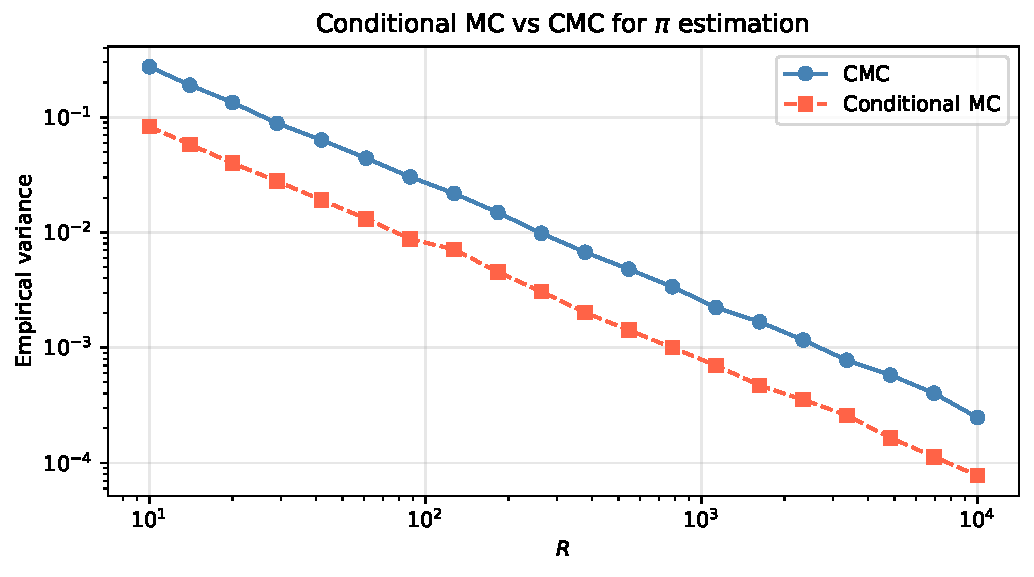
\includegraphics[width=0.72\textwidth]{fig_conditional_mc}
  \end{center}
  \small
  The conditional MC estimator consistently achieves lower variance.
  Both converge at rate $1/R$, but CMC has a higher constant.
\end{frame}

% ──────────────────────────────────────────────────────────────────────────────
\subsection{5.1.7 Importance Sampling}
% ──────────────────────────────────────────────────────────────────────────────

\begin{frame}[allowframebreaks]{5.1.7 Importance Sampling}

  \begin{block}{Change of Measure}
    Goal: estimate $I = \int_E k(x) f(x)\, dx = \mathbb{E}_f[k(X)]$.
    Let $\tilde{f}(x)$ be a \emph{proposal density} (positive where $f>0$).
    Then:
    \[
      I = \int_E k(x)\frac{f(x)}{\tilde{f}(x)}\tilde{f}(x)\,dx
        = \mathbb{E}_{\tilde{f}}\!\left[k(\tilde{X})\frac{f(\tilde{X})}{\tilde{f}(\tilde{X})}\right]
    \]
  \end{block}

  \begin{block}{Importance Sampling Estimator}
    \[
      \hat{Y}_R^{\mathrm{IS}} = \frac{1}{R}\sum_{j=1}^R k(\tilde{X}_j)\frac{f(\tilde{X}_j)}{\tilde{f}(\tilde{X}_j)}
    \]
    where $\tilde{X}_1, \ldots, \tilde{X}_R \overset{\text{iid}}{\sim} \tilde{f}$.\\[2pt]
    The ratio $L(x) = f(x)/\tilde{f}(x)$ is called the \emph{likelihood ratio}.
  \end{block}

  \framebreak

  \begin{block}{Variance of IS Estimator}
    \[
      \mathrm{Var}(\hat{Y}_R^{\mathrm{IS}}) = \frac{1}{R}
      \left[\int_E \left(k(x)\frac{f(x)}{\tilde{f}(x)}\right)^2 \tilde{f}(x)\,dx - I^2\right]
    \]
  \end{block}

  \begin{block}{Optimal Proposal Distribution}
    The zero-variance proposal is:
    \[
      g^*(x) = \frac{k(x)f(x)}{\int_E k(x)f(x)\,dx} = \frac{k(x)f(x)}{I}
    \]
    (impractical, since it requires knowing $I$; but guides the choice of $\tilde{f}$).
  \end{block}

  \begin{block}{Proposition 5.1.33 -- CLT for IS}
    $\hat{Y}_R^{\mathrm{IS}}$ is unbiased and strongly consistent, and:
    \[
      \sqrt{R}(\hat{Y}_R^{\mathrm{IS}} - I) \xrightarrow{\mathcal{D}} \mathcal{N}(0, \varsigma^2)
    \]
    where $\varsigma^2 = \int_E (k(x)f(x)/\tilde{f}(x))^2\tilde{f}(x)\,dx - I^2$.
  \end{block}

  \framebreak

  \textbf{Example 5.1.34 -- $I = \mathbb{P}(X > 2)$ for Cauchy $X$:}
  \begin{itemize}
    \item CMC: $\mathrm{Var}(\hat{Y}_R^{\mathrm{CMC}}) = I(1-I)/R = 0.1258/R$
    \item IS with $\tilde{f}(x) = 2/x^2 \cdot \mathbf{1}(x>2)$:
          $\mathrm{Var}(\hat{Y}_R^{\mathrm{IS}}) = 9.55\times10^{-5}/R$
    \item Reduction: $\approx 1317\times$
  \end{itemize}

  \medskip
  \textbf{Example 5.1.36 -- $I = \mathbb{P}(X > 4)$ for $X \sim \mathcal{N}(0,1)$:}
  \begin{itemize}
    \item $I \approx 3.167 \times 10^{-5}$
    \item CMC: $\mathrm{Var} = I(1-I)/R \approx 3.167 \times 10^{-5}/R$
    \item IS with $\tilde{f} = \mathcal{N}(4,1)$:
          $\mathrm{Var}(Y_1^{\mathrm{IS}}) = 3.601\times10^{-8}$
    \item Reduction: $\approx 879 \times$
  \end{itemize}

\end{frame}

\begin{frame}[fragile]{5.1.7 Importance Sampling -- Python Code}
\begin{lstlisting}[style=python]
import numpy as np
from scipy.stats import norm

def IS_normal_tail(theta, R=100000):
    """Estimate P(Z > 4), Z~N(0,1) using IS with N(theta, 1) proposal."""
    Z_tilde = np.random.normal(theta, 1, R)
    # Likelihood ratio: phi(z; 0,1) / phi(z; theta, 1)
    log_LR   = -theta * Z_tilde + theta**2 / 2
    Y_IS     = (Z_tilde > 4) * np.exp(log_LR)
    return np.mean(Y_IS), np.var(Y_IS) / R

np.random.seed(42)
true_I = 1 - norm.cdf(4)
print(f"True P(Z>4) = {true_I:.2e}")

for theta in [0, 2, 4, 4.2256]:
    est, var = IS_normal_tail(theta)
    print(f"  theta={theta:.4f}: est={est:.2e}, var={var:.2e}, "
          f"reduction={true_I*(1-true_I)/var:.1f}x")
\end{lstlisting}
\end{frame}

\begin{frame}{5.1.7 Importance Sampling -- Proposal Distributions}
  \begin{center}
    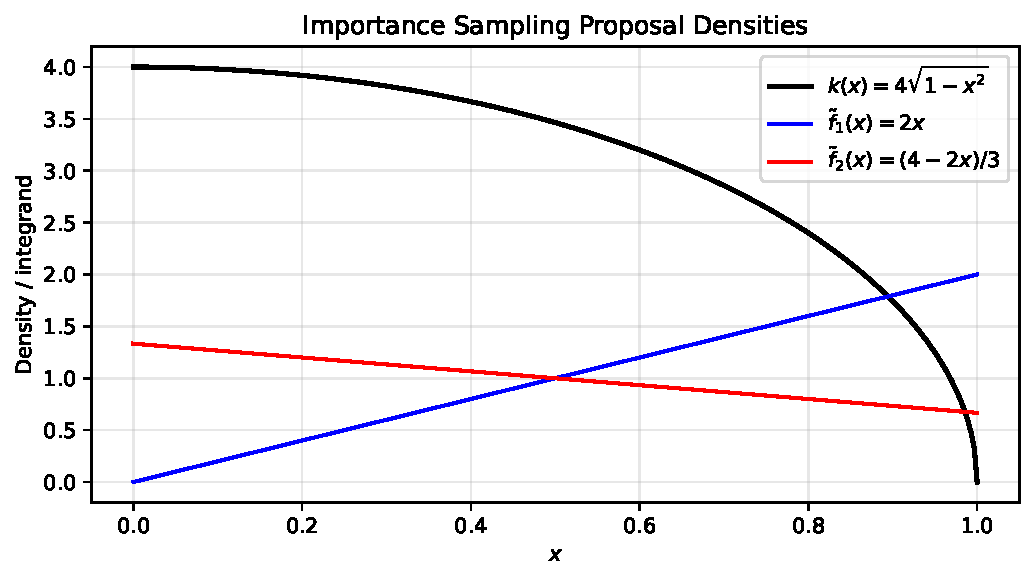
\includegraphics[width=0.72\textwidth]{fig_IS_proposals}
  \end{center}
  \small
  The optimal proposal $\tilde{f} \propto k(x)f(x)$ should closely
  match the shape of the integrand. Among $\tilde{f}_1 = 2x$ and
  $\tilde{f}_2 = (4-2x)/3$, the one closer to $k(x)$ achieves lower variance.
\end{frame}

\begin{frame}{5.1.7 IS for Rare Events: $\mathbb{P}(Z>4)$}
  \begin{center}
    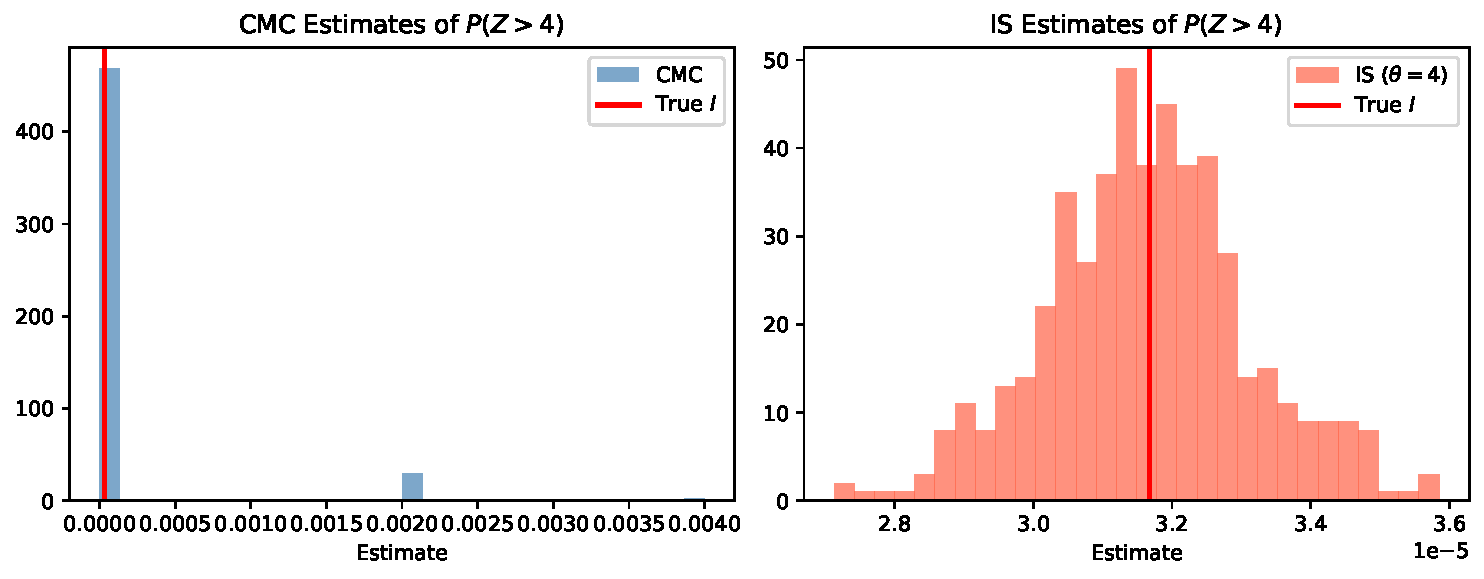
\includegraphics[width=0.82\textwidth]{fig_IS_rare_event}
  \end{center}
  \small
  CMC estimates are mostly 0 (the event rarely occurs). IS with $\tilde{f} = \mathcal{N}(4,1)$
  concentrates samples in the rare-event region, giving consistent estimates.
\end{frame}

% ──────────────────────────────────────────────────────────────────────────────
\subsection{5.1.7 (cont.) Self-Normalised IS and Likelihood Ratio}
% ──────────────────────────────────────────────────────────────────────────────

\begin{frame}[allowframebreaks]{Self-Normalised Importance Sampling}

  \begin{block}{When normalisation is unknown}
    If $f(x) = c \cdot f_0(x)$ and $\tilde{f}(x) = \tilde{c} \cdot \tilde{f}_0(x)$
    with unknown constants, define $w(x) = f_0(x)/\tilde{f}_0(x)$ and:
    \[
      I = \frac{\mathbb{E}_{\tilde{f}}[k(\tilde{X})w(\tilde{X})]}
               {\mathbb{E}_{\tilde{f}}[w(\tilde{X})]}
    \]
    \[
      \hat{Y}_R = \frac{\sum_{i=1}^R k(\tilde{X}_i)w(\tilde{X}_i)}
                       {\sum_{i=1}^R w(\tilde{X}_i)}
    \]
    This is the \emph{self-normalised} (or ratio) IS estimator.
  \end{block}

  \begin{block}{Estimated Variance (Delta Method)}
    \[
      \widehat{\mathrm{Var}}(\hat{Y}_R) = \sum_{i=1}^R (w'(\tilde{X}_i))^2
      (k(\tilde{X}_i) - \hat{Y}_R)^2
    \]
    where $w'(\tilde{X}_i) = w(\tilde{X}_i)/\sum_j w(\tilde{X}_j)$.
  \end{block}

  \framebreak

  \begin{block}{Likelihood Ratio (Proposition 5.1.42)}
    Under two probability measures $\mathbb{P}$ and $\tilde{\mathbb{P}}$ with
    $X_1, X_2, \ldots$ i.i.d.\ with densities $f$ and $\tilde{f}$:
    \[
      L_n = \prod_{j=1}^n \frac{f(X_j)}{\tilde{f}(X_j)}
    \]
    then $\mathbb{P}(d\omega) = L_n(\omega)\tilde{\mathbb{P}}(d\omega)$, and
    for any integrable $Y$: $I = \mathbb{E}_f Y = \tilde{\mathbb{E}}[Y L_n]$.
  \end{block}

  \begin{block}{Exponential Change of Measure (Rare Events)}
    For $X_i$ with p.d.f.\ $f(x)$, define $f_\theta(x) = e^{\theta x}f(x)/M(\theta)$
    where $M(\theta) = \mathbb{E}[e^{\theta X}]$. Then:
    \[
      I(n) = \mathbb{P}(S_n > n(\mu+\varepsilon))
           = \mathbb{E}_\theta\!\left[\mathbf{1}_{S_n > n(\mu+\varepsilon)}
             e^{-\theta S_n + n\kappa(\theta)}\right]
    \]
    Choose $\theta = \theta_0$ such that $\kappa'(\theta_0) = \mu + \varepsilon$
    for the logarithmically efficient estimator.
  \end{block}

\end{frame}

\begin{frame}{5.1.7 Self-Normalised IS Weights}
  \begin{center}
    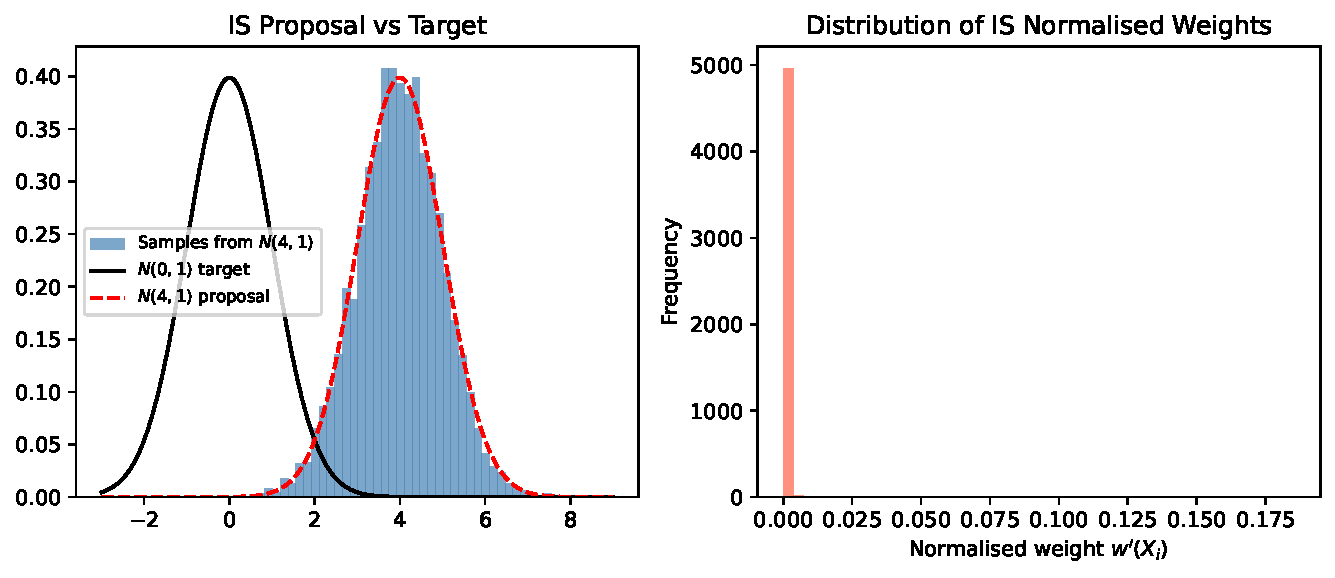
\includegraphics[width=0.82\textwidth]{fig_snIS_weights}
  \end{center}
  \small
  Using a proposal $N(4,1)$ concentrates samples in the rare region.
  The resulting normalised weights $w'(X_i)$ have low variance, ensuring
  a stable estimator.
\end{frame}

% ──────────────────────────────────────────────────────────────────────────────
\subsection{5.1.8 Cross-Entropy Method}
% ──────────────────────────────────────────────────────────────────────────────

\begin{frame}[allowframebreaks]{5.1.8 The Cross-Entropy Method}

  \begin{block}{Motivation}
    How to choose the best proposal $\tilde{f}_\theta$ from a parametric family
    $\{\tilde{f}_\theta : \theta \in \Theta\}$?
  \end{block}

  \begin{block}{KL Divergence and Optimal $\theta^*$}
    Minimise the Kullback-Leibler divergence from $g^*(x) = k(x)f(x)/I$
    to $\tilde{f}_\theta$:
    \[
      \theta^* = \arg\max_\theta \int k(\mathbf{x})\log\tilde{f}_\theta(\mathbf{x})
      f(\mathbf{x})\,d\mathbf{x}
      = \arg\max_\theta \mathbb{E}_f\!\left[k(\mathbf{X})\log\tilde{f}_\theta(\mathbf{X})\right]
    \]
    Estimated from $M$ samples as:
    \[
      \hat{\theta}^* = \arg\max_\theta \frac{1}{M}\sum_{i=1}^M
      k(\mathbf{X}_i)\log\tilde{f}_\theta(\mathbf{X}_i)
    \]
  \end{block}

  \framebreak

  \begin{block}{CE Method for Rare Event Simulation}
    For $I = \mathbb{P}_f(h(\mathbf{X}) \ge \gamma)$, iteratively:
    \begin{enumerate}
      \item Update level: $\gamma_t = $ $(1-\rho)$-quantile of $h(\mathbf{X}_i)$
      \item Update parameter using likelihood ratio $L(\mathbf{X}, f, f_{\theta'_{t-1}})$:
            \[
              \theta'_t = \arg\max_\theta \frac{1}{M}\sum_{i=1}^M
              \mathbf{1}(h(\mathbf{X}_i) \ge \gamma_t)
              L(\mathbf{X}_i, f, f_{\theta'_{t-1}})\log f_\theta(\mathbf{X}_i)
            \]
      \item Apply \emph{smoothing}: $\theta'_t := \alpha\theta'_t + (1-\alpha)\theta'_{t-1}$
      \item Stop when $\gamma_t \ge \gamma$; final IS estimator:
            \[
              \hat{Y}_R^{\mathrm{CE}} = \frac{1}{R}\sum_{i=1}^R
              \mathbf{1}(h(\mathbf{X}_i) > \gamma)L(\mathbf{X}_i, f, f_{\theta_T})
            \]
    \end{enumerate}
  \end{block}

  \framebreak

  \begin{block}{CE Update for Normal Family $\tilde{f}_\theta = \mathcal{N}(\theta, \Sigma)$}
    The optimal parameter update is a weighted mean:
    \[
      \theta'_t = \frac{\sum_{i=1}^M \mathbf{1}(h(\mathbf{X}_i)\ge\gamma_t)
      w_{i,t-1}\mathbf{X}_i}{\sum_{i=1}^M \mathbf{1}(h(\mathbf{X}_i)\ge\gamma_t) w_{i,t-1}}
    \]
    where $w_{i,t-1} = L(\mathbf{X}_i, f, f_{\theta'_{t-1}})$.
  \end{block}

  \textbf{Example 5.1.47 -- $\mathbb{P}(X>4)$ for $X\sim\mathcal{N}(0,1)$:}
  \begin{itemize}
    \item CE with $\{\mathcal{N}(\theta,1)\}$ family: $\theta^* = 4.2256$
    \item $\mathrm{Var}(\hat{Y}_R^{\mathrm{IS}})$ at $\theta=4$: $3.601\times10^{-8}$
    \item At CE $\theta^*=4.2256$: $4.516\times10^{-9}$ (better by $8\times$)
    \item Algorithm converged in 46 steps (Example 5.1.54)
  \end{itemize}

\end{frame}

\begin{frame}[fragile]{5.1.8 Cross-Entropy Method -- Python Code}
\begin{lstlisting}[style=python]
import numpy as np

def CE_normal_1D(M=10000, rho=0.05, alpha=0.4, gamma_target=4.0):
    """Cross-entropy method to estimate P(Z > 4), Z~N(0,1)."""
    theta = 0.0
    for t in range(100):
        X = np.random.normal(theta, 1, M)
        # Likelihood ratio to original N(0,1)
        w = np.exp(-theta * X + theta**2 / 2)
        # Update level (1-rho quantile)
        gamma_t = np.quantile(X, 1 - rho)
        # Update theta: weighted mean of X satisfying h(X) >= gamma_t
        mask = X >= gamma_t
        if mask.sum() > 0:
            new_theta = np.sum(w[mask] * X[mask]) / np.sum(w[mask])
            theta = alpha * new_theta + (1 - alpha) * theta
        print(f"t={t+1}: gamma={gamma_t:.3f}, theta={theta:.4f}")
        if gamma_t >= gamma_target:
            break
    return theta

theta_CE = CE_normal_1D()
print(f"\nCE theta* = {theta_CE:.4f}  (theory: 4.2256)")
\end{lstlisting}
\end{frame}

\begin{frame}{5.1.8 Cross-Entropy Convergence}
  \begin{center}
    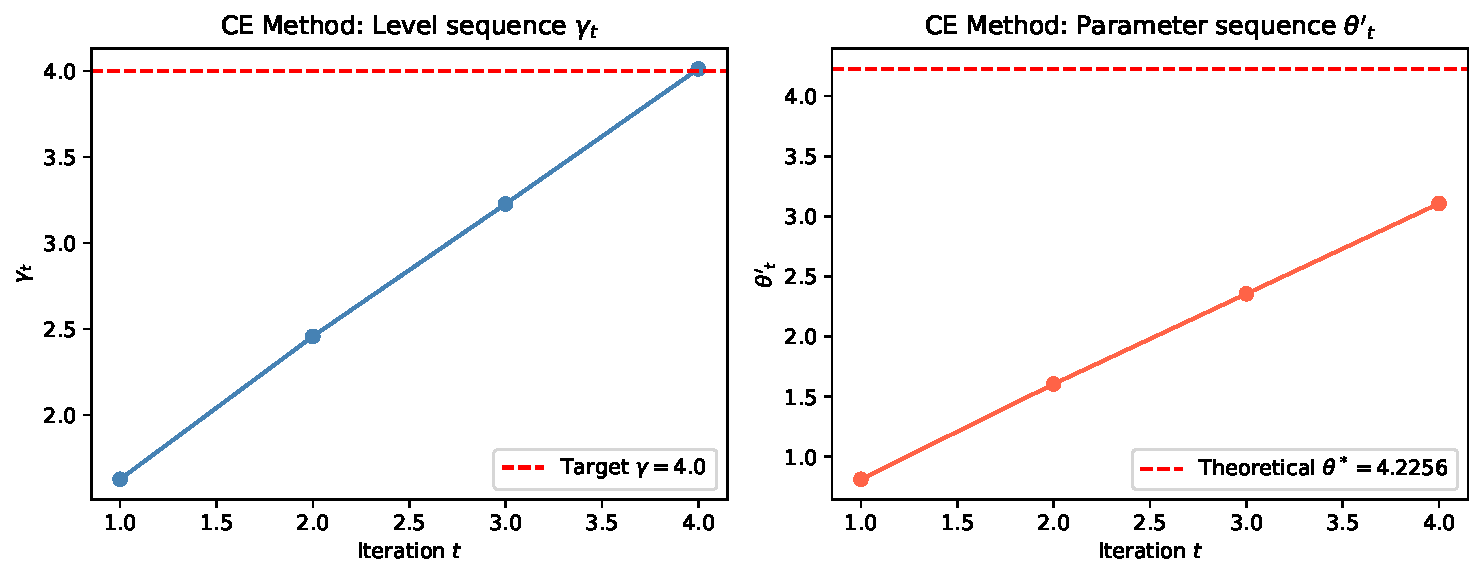
\includegraphics[width=0.85\textwidth]{fig_CE_convergence}
  \end{center}
  \small
  Left: Level sequence $\gamma_t$ converges to target $\gamma=4$.
  Right: Parameter $\theta'_t$ converges to theoretical optimum $\theta^*=4.2256$.
\end{frame}

% ──────────────────────────────────────────────────────────────────────────────
\subsection{5.1.9 Summary: Reducing Variance for Estimating pi}
% ──────────────────────────────────────────────────────────────────────────────

\begin{frame}{5.1.9 Summary: Estimating $\pi$ -- Variance Comparison}

  \begin{center}
    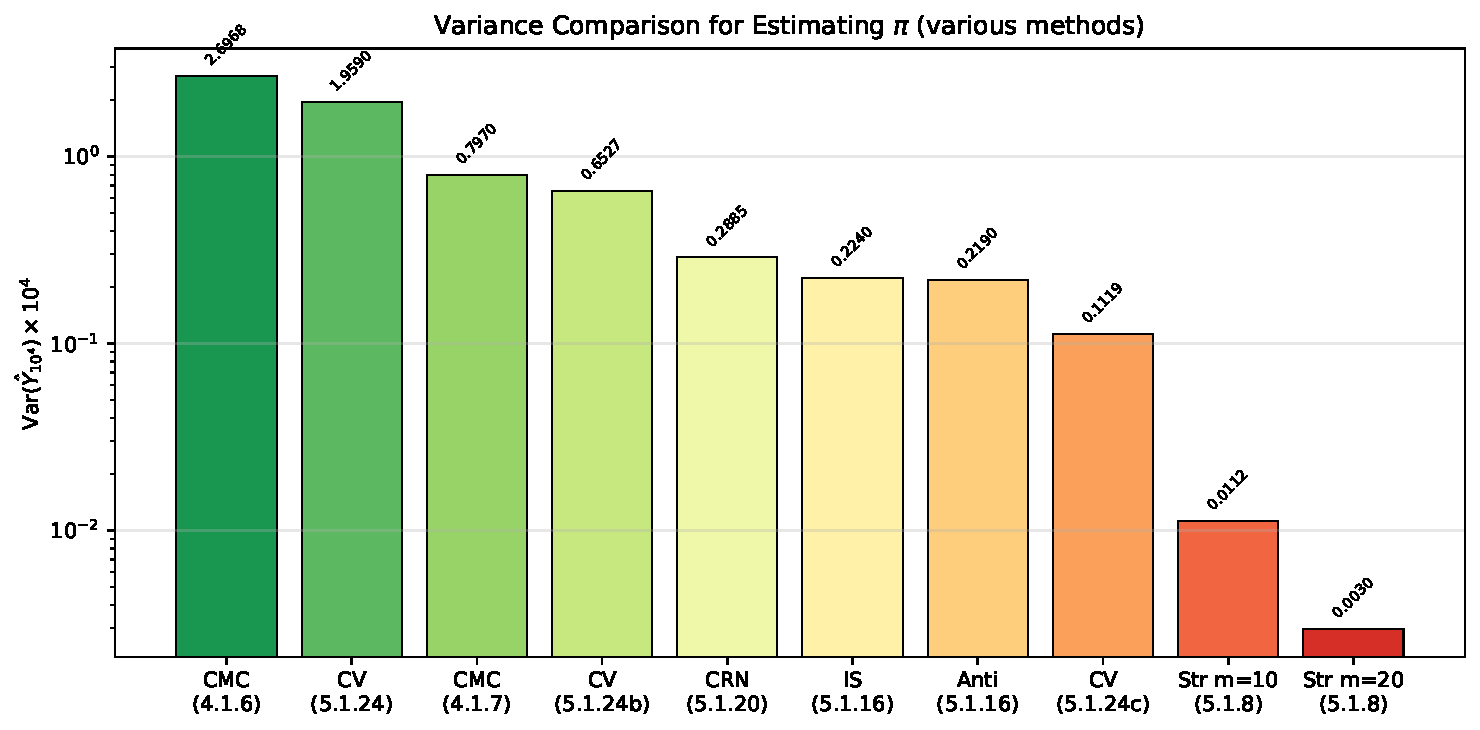
\includegraphics[width=0.82\textwidth]{fig_variance_summary}
  \end{center}

\end{frame}

\begin{frame}{5.1.9 Summary Table (from Table 5.11)}
  \small
  \begin{tabular}{llcl}
    \toprule
    Method & Description & $\mathrm{Var}(\hat{Y}_{10^4})\!\times\!10^4$ & Reduction \\
    \midrule
    CMC    & $Y=4\mathbf{1}(U_1^2+U_2^2\le1)$                           & 2.697  & $1\times$ \\
    CV     & $X=\mathbf{1}(U_1+U_2\le1)$                                  & 1.959  & $1.4\times$ \\
    CMC    & $Y=4\sqrt{1-U^2}$                                             & 0.797  & $3.4\times$ \\
    CV     & $X=\mathbf{1}(U_1+U_2\ge\sqrt{2})$                          & 0.653  & $4.1\times$ \\
    CRN    & $Y=8/(1+U^2)-4\sqrt{1-U^2}$                                  & 0.289  & $9.3\times$ \\
    IS     & $\tilde{f}=(4-2x)/3$                                          & 0.224  & $12\times$ \\
    Anti   & $Y_1=4\sqrt{1-U^2}$, $Y_2=4\sqrt{1-(1-U)^2}$               & 0.219  & $12\times$ \\
    CV     & poly. $X$, 4th degree                                         & 0.112  & $24\times$ \\
    Str    & $m=10$ strata, optimal                                        & 0.0112 & $240\times$ \\
    Str    & $m=20$ strata, optimal                                        & 0.00296 & $911\times$ \\
    \bottomrule
  \end{tabular}
\end{frame}

% ==============================================================================
\section{5.2 Finance and Actuarial Applications}
% ==============================================================================

\begin{frame}{5.2 Finance and Actuarial Science -- Overview}

  \begin{block}{Motivation}
    Classical financial mathematics is built on \emph{geometric Brownian motion}
    (GBM). Options pricing requires computing expectations of functionals of GBM.
    Variance reduction techniques can dramatically reduce the computational cost.
  \end{block}

  \medskip
  \textbf{Topics covered:}
  \begin{enumerate}
    \item Brownian motion: definition, simulation, bisection method
    \item Financial contracts: European/Asian options, Black-Scholes
    \item Stratified sampling for option pricing
    \item Control variates for options
    \item Antithetic variates for options
    \item Importance sampling for options
  \end{enumerate}

\end{frame}

% ──────────────────────────────────────────────────────────────────────────────
\subsection{5.2.1 Brownian Motion}
% ──────────────────────────────────────────────────────────────────────────────

\begin{frame}[allowframebreaks]{5.2.1 Brownian Motion and Related Processes}

  \begin{block}{Definition 5.2.1 -- Standard Brownian Motion}
    A stochastic process $(B(t): t \in [0,T])$ is a \emph{standard Brownian motion} if:
    \begin{itemize}
      \item[(i)] $B(0) = 0$
      \item[(ii)] Increments $B(t_1), B(t_2)-B(t_1), \ldots, B(t_n)-B(t_{n-1})$
                 are independent for all $0 \le t_1 < \cdots < t_n \le T$
      \item[(iii)] $B(t_2) - B(t_1) \sim \mathcal{N}(0, t_2-t_1)$ for $0 \le t_1 \le t_2$
      \item[(iv)] $t \mapsto B(t)$ is continuous a.s.
    \end{itemize}
  \end{block}

  \begin{block}{Proposition 5.2.2 -- Characterisation}
    A process with a.s.\ continuous trajectories is a standard BM iff:
    \[
      \mathrm{Cov}(B(s), B(t)) = \min(s, t), \quad \text{for all } 0 \le s \le t \le T.
    \]
  \end{block}

  \framebreak

  \begin{block}{Simulation: Algorithm 36}
    On grid $t_i = i\Delta$, $\Delta = 1/N$, generate
    $Z_1, \ldots, Z_N \overset{\text{iid}}{\sim} \mathcal{N}(0,1)$:
    \[
      B(i\Delta) = \sum_{k=1}^i \sqrt{\Delta}\, Z_k
    \]
  \end{block}

  \begin{block}{Brownian Motion with Drift}
    \[
      X(t) = \sigma B(t) + \mu t, \qquad \mu \in \mathbb{R},\ \sigma > 0
    \]
  \end{block}

  \begin{block}{Geometric Brownian Motion (GBM)}
    \[
      S(t) = S(0)\exp\!\left(\left(r - \frac{\sigma^2}{2}\right)t + \sigma B(t)\right)
    \]
    where $r$ is the risk-free rate and $\sigma$ the volatility.
  \end{block}

  \framebreak

  \begin{block}{Brownian Bridge (Bisection)}
    The \emph{Brownian bridge} is BM conditioned on $B(1)=0$.
    Given $B(0)=0$ and $B(1)=y$, the midpoint $B(1/2)$ satisfies:
    \[
      (B(1/2) \mid B(1) = y) \sim \mathcal{N}(y/2,\, 1/4)
    \]
    This allows the \emph{bisection algorithm} (Algorithm 38) that generates
    BM in order: $B(1), B(1/2), B(1/4), B(3/4), \ldots$
    Useful for stratified sampling of BM.
  \end{block}

\end{frame}

\begin{frame}[fragile]{5.2.1 Brownian Motion -- Python Code}
\begin{lstlisting}[style=python]
import numpy as np
import matplotlib.pyplot as plt

def sim_brownian(N=1000, T=1.0, n_paths=5):
    """Simulate Brownian motion on [0,T] with N steps."""
    dt   = T / N
    t    = np.linspace(0, T, N+1)
    paths = np.zeros((n_paths, N+1))
    for i in range(n_paths):
        Z = np.random.standard_normal(N)
        paths[i, 1:] = np.cumsum(np.sqrt(dt) * Z)
    return t, paths

def sim_gbm(S0=100, r=0.05, sigma=0.25, N=252, n_paths=5):
    """Simulate Geometric Brownian Motion (risk-neutral)."""
    dt    = 1.0 / N
    mu    = r - sigma**2 / 2
    t     = np.linspace(0, 1, N+1)
    paths = np.zeros((n_paths, N+1))
    paths[:, 0] = S0
    for i in range(n_paths):
        Z = np.random.standard_normal(N)
        log_ret = mu * dt + sigma * np.sqrt(dt) * Z
        paths[i, 1:] = S0 * np.exp(np.cumsum(log_ret))
    return t, paths
\end{lstlisting}
\end{frame}

\begin{frame}{5.2.1 Brownian Motion Sample Paths}
  \begin{columns}
    \begin{column}{0.5\textwidth}
      \centering
      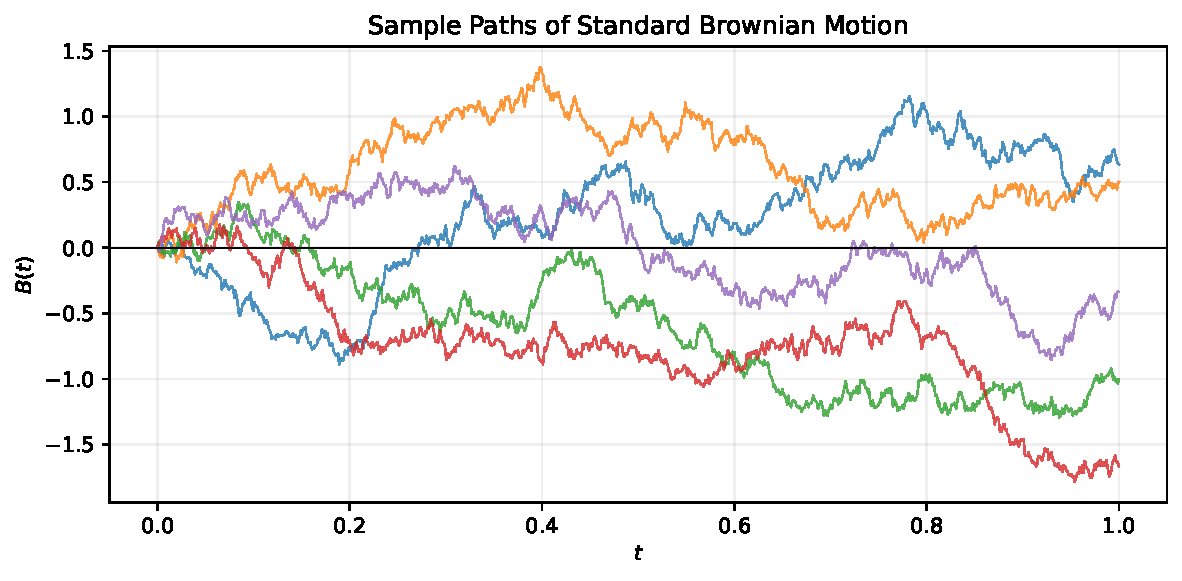
\includegraphics[width=\textwidth]{fig_brownian_motion}
      \small Standard BM $B(t)$
    \end{column}
    \begin{column}{0.5\textwidth}
      \centering
      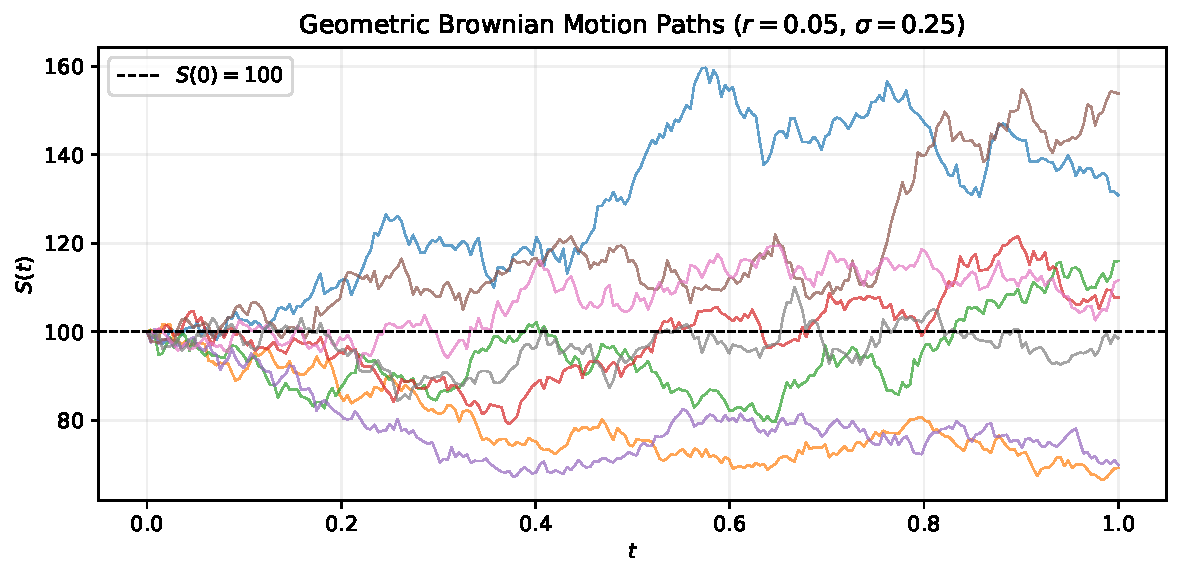
\includegraphics[width=\textwidth]{fig_geometric_brownian}
      \small GBM $S(t) = S(0)\exp(\mu^* t + \sigma B(t))$
    \end{column}
  \end{columns}
\end{frame}

% ──────────────────────────────────────────────────────────────────────────────
\subsection{5.2.2 Financial Contracts}
% ──────────────────────────────────────────────────────────────────────────────

\begin{frame}[allowframebreaks]{5.2.2 Financial Contracts and Black-Scholes}

  \textbf{Common option types (under GBM($r,\sigma$)):}
  \begin{itemize}
    \item \textbf{European call}: $f(S(1)) = (S(1)-K)_+$
    \item \textbf{European put}: $f(S(1)) = (K-S(1))_+$
    \item \textbf{Asian call}: $f = \left(\frac{1}{n}\sum_{j=1}^n S(j/n) - K\right)_+$
    \item \textbf{Up-and-out call}: $(S(1)-K)_+ \cdot \mathbf{1}(S(t) < b\ \forall t)$
    \item \textbf{European basket call}: $\left(\sum_{j=1}^d w_j S_j(1) - K\right)_+$
  \end{itemize}

  \begin{block}{Option Price under Risk-Neutral Measure}
    \[
      I = e^{-r}\mathbb{E}\!\left[f(S(t_1), \ldots, S(t_n))\right]
    \]
    where $S(t) = S(0)\exp\!\left(\mu^* t + \sigma B(t)\right)$,
    $\mu^* = r - \sigma^2/2$.
  \end{block}

  \framebreak

  \begin{block}{Black-Scholes Formula (European Call)}
    \[
      \mathbb{E}(S(1)-K)_+ = S(0)\Phi(d_1) - Ke^{-r}\Phi(d_2)
    \]
    \[
      d_1 = \frac{1}{\sigma}\!\left[\log\!\left(\frac{S(0)}{K}\right) + r + \frac{\sigma^2}{2}\right],
      \quad d_2 = d_1 - \sigma
    \]
    where $\Phi$ is the standard normal CDF.
  \end{block}

  \textbf{Example parameters (used throughout):}
  \begin{itemize}
    \item $r = 0.05$, $\sigma = 0.25$, $S(0) = 100$, $K = 100$
    \item $\mu^* = r - \sigma^2/2 = -0.01875$
    \item Exact Black-Scholes price $I \approx 12.336$
  \end{itemize}

\end{frame}

\begin{frame}{5.2.2 Black-Scholes vs Monte Carlo}
  \begin{center}
    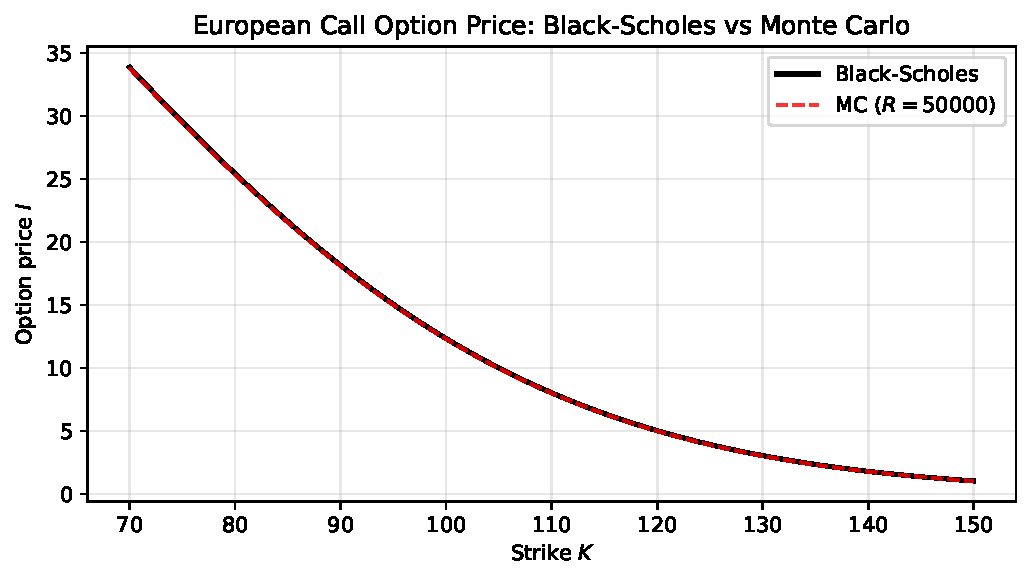
\includegraphics[width=0.72\textwidth]{fig_black_scholes}
  \end{center}
  \small
  Black-Scholes formula gives exact option prices; Monte Carlo
  approximates them with controlled statistical error.
\end{frame}

% ──────────────────────────────────────────────────────────────────────────────
\subsection{5.2.3 Stratified Sampling for Finance}
% ──────────────────────────────────────────────────────────────────────────────

\begin{frame}[allowframebreaks]{5.2.3 Stratified Sampling for Finance}

  \textbf{Example 5.2.5 -- European Call Option, $m$ strata:}

  \begin{block}{Method}
    Stratify on $B(1) \sim \mathcal{N}(0,1)$: strata $A_j = (a_{j-1}, a_j]$
    where $a_j = \Phi^{-1}(j/m)$.
    \begin{itemize}
      \item Proportional allocation: $R_j = R/m$
      \item Optimal allocation: $R_j \propto \hat{\sigma}_j$ (from pilot)
    \end{itemize}
  \end{block}

  \textbf{Results (Table 5.13)} with $R=10^5$, $S(0)=100$, $r=0.05$, $\sigma=0.25$, $K=100$:
  \begin{center}
    \small
    \begin{tabular}{rcccc}
      \toprule
      Strata $m$ & CMC & 5 & 50 & 200 \\
      \midrule
      Estimate & 12.280 & 12.351 & 12.338 & 12.336 \\
      Error $b$ & 0.115 & 0.043 & 0.025 & 0.002 \\
      Var reduction & -- & 7.2 & 21.0 & 3778 \\
      \bottomrule
    \end{tabular}
  \end{center}

  \framebreak

  \textbf{Example 5.2.8 -- Asian Call Option with Stratified BM:}
  Two methods for stratifying:
  \begin{enumerate}
    \item \textbf{Method 1}: Stratify on $(B(1/n), \ldots, B(n/n))$ using
          multivariate normal strata (concentric ellipses via $\chi^2$ distribution)
    \item \textbf{Method 2}: Stratify $Z_{2^k}$ and $Z_{2^{k-1}}$ in bisection
          algorithm; resulting in $m^2$ strata for $(B(1/2), B(1))$
  \end{enumerate}

  Results with $K=100$: $m=200$ strata reduces variance by factor $84\times$.

\end{frame}

% ──────────────────────────────────────────────────────────────────────────────
\subsection{5.2.4 Control Variates for Options}
% ──────────────────────────────────────────────────────────────────────────────

\begin{frame}[allowframebreaks]{5.2.4 Control Variates for Options Pricing}

  \textbf{Example 5.2.9 -- Asian Call Option:}
  \[
    I = e^{-r}\mathbb{E}(A - K)_+, \quad A = \frac{1}{n}\sum_{j=1}^n S(j/n)
  \]

  \begin{block}{Control Variate: Geometric Mean}
    The geometric mean $G = \left(\prod_{j=1}^n S(j/n)\right)^{1/n}$
    follows a log-normal distribution with exact analytical mean:
    \[
      G = S(0)\exp\!\left[\mu_N + \sigma_N Z\right]
    \]
    where $\mu_N = \mu^*(n+1)/(2n)$,
    $\sigma_N^2 = \sigma^2(n+1)(2n+1)/(6n^2)$,
    and $Z \sim \mathcal{N}(0,1)$.\\[2pt]
    Control variate: $W = e^{-r}\mathbb{E}(G-K)_+$ (computed via Black-Scholes).
  \end{block}

  \framebreak

  \textbf{Results (Table 5.17)} with $R=10^4$, $n=10$, $K=100$, $r=0.05$:
  \begin{center}
    \small
    \begin{tabular}{rcccc}
      \toprule
      $K$ & CMC error & CV error & Reduction & Anti error \\
      \midrule
      150 & 2.45  & 0.374 & $\approx 40\times$ & 0.0153 \\
      120 & 10.5  & 0.586 & $\approx 320\times$ & 0.0943 \\
      100 & 21.5  & 0.731 & $\approx 870\times$ & 2.10   \\
       50 & 30.7  & 0.998 & -- & 0.302  \\
      \bottomrule
    \end{tabular}
  \end{center}

  The CV estimator dramatically reduces error for out-of-the-money options.

\end{frame}

% ──────────────────────────────────────────────────────────────────────────────
\subsection{5.2.5 Antithetic Variates for Options}
% ──────────────────────────────────────────────────────────────────────────────

\begin{frame}[allowframebreaks]{5.2.5 Antithetic Variates for Options}

  \textbf{Example 5.2.10 -- Asian Call with Antithetic Variates:}

  \begin{block}{Construction}
    Generate $Z_1, \ldots, Z_n \overset{\text{iid}}{\sim} \mathcal{N}(0,1)$,
    compute original path $B(k/n) = n^{-1/2}\sum_{j=1}^k Z_j$,
    and antithetic path $B'(k/n) = n^{-1/2}\sum_{j=1}^k(-Z_j)$:
    \[
      \hat{Y}_R^{\mathrm{anti}} = \frac{1}{2R}\sum_{j=1}^R
      \left[e^{-r}(A_j - K)_+ + e^{-r}(A'_j - K)_+\right]
    \]
  \end{block}

  \textbf{Key insight:} $S(t)$ is a monotone increasing function of $B(t)$,
  and $A$ is a monotone function of $S$, so antithetic variates guarantee
  $\mathrm{Cov}(Y, Y') < 0$.

  \framebreak

  \textbf{Comparison with CMC and CV (Table 5.17):}
  \begin{itemize}
    \item For $K=150$: antithetic error = 0.0153 vs CMC error = 2.45
          (reduction $\approx 25\,000\times$ in variance!)
    \item For $K=120$: antithetic error = 0.0943 vs CMC error = 10.5
    \item Antithetic outperforms CV for deep out-of-the-money options
  \end{itemize}

\end{frame}

\begin{frame}{5.2.5 Antithetic Variates -- Path Illustration}
  \begin{center}
    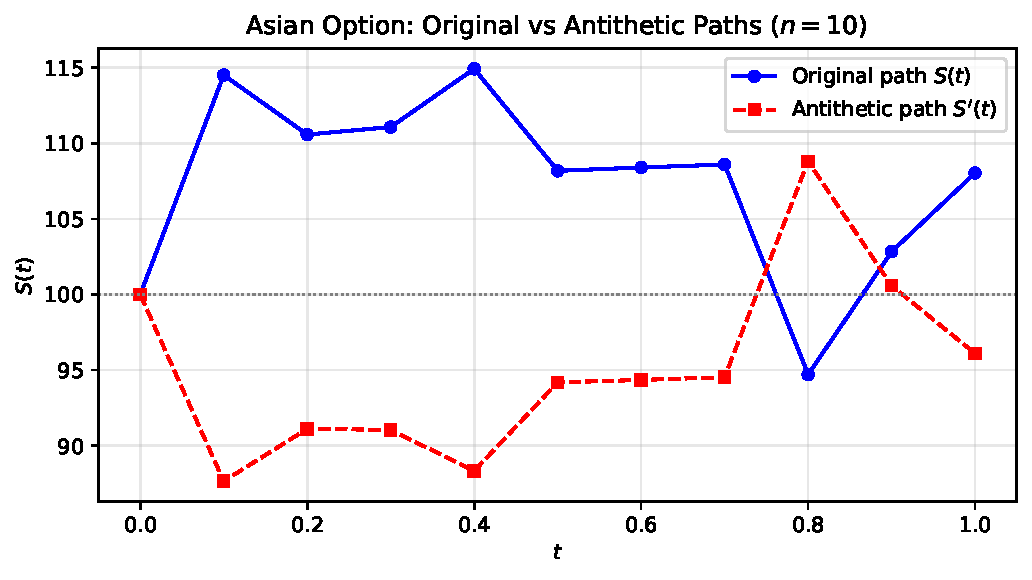
\includegraphics[width=0.72\textwidth]{fig_asian_option_antithetic}
  \end{center}
  \small
  The antithetic path $S'(t) = S(0)\exp(\mu^* t - \sigma B(t))$ mirrors
  the original. When $S(t)$ tends up, $S'(t)$ tends down, creating
  negative correlation in payoffs.
\end{frame}

% ──────────────────────────────────────────────────────────────────────────────
\subsection{5.2.6 Importance Sampling for Options}
% ──────────────────────────────────────────────────────────────────────────────

\begin{frame}[allowframebreaks]{5.2.6 Importance Sampling for Options}

  \textbf{Example 5.2.11 -- European Call, IS with $\tilde{f} = \mathcal{N}(x^*, 1)$:}

  \begin{block}{IS Estimator}
    Rewrite: $I = e^{-r}\int_{-\infty}^\infty (S(0)e^{\mu^*+\sigma z}-K)_+\phi_{0,1}(z)\,dz$.
    Use proposal $\phi_{x^*,1}(z)$. IS estimator:
    \[
      \hat{Y}_R^{\mathrm{IS}} = \frac{1}{R}\sum_{i=1}^R
      e^{-r}(S(0)e^{\mu^*+\sigma\tilde{Z}_i}-K)_+ e^{-x^*\tilde{Z}_i+(x^*)^2/2}
    \]
    where $\tilde{Z}_i \sim \mathcal{N}(x^*, 1)$.
  \end{block}

  \begin{block}{Two Methods for Choosing $x^*$}
    \begin{itemize}
      \item \textbf{Heuristic}: $x^* = \arg\sup_z h(z)$ where
            $h(z) = (S(0)e^{\mu^*+\sigma z}-K)_+\phi_{0,1}(z)$
            $\Rightarrow$ solve $S(0)\sigma e^{\mu^*+\sigma z} - z(S(0)e^{\mu^*+\sigma z}-K) = 0$
      \item \textbf{CE method}: $\hat{x}^*_{\mathrm{CE}} = \frac{\sum_i Z_i(S(0)e^{\mu^*+\sigma Z_i}-K)_+}{\sum_i(S(0)e^{\mu^*+\sigma Z_i}-K)_+}$
    \end{itemize}
  \end{block}

  \framebreak

  \textbf{Results (Table 5.18)} with $S(0)=K=100$, $r=0.05$, $\sigma=0.25$:
  \begin{center}
    \small
    \begin{tabular}{lccc}
      \toprule
              & CMC    & IS ($x^*=1.033$) & IS CE ($x^*=1.232$) \\
      \midrule
      Estimate & 12.391 & 12.302 & 12.306 \\
      Error $b$ & 0.387 & 0.125 & 0.120 \\
      Var reduction & -- & 9.65 & 10.46 \\
      \bottomrule
    \end{tabular}
  \end{center}

  Both IS methods achieve $\approx 10\times$ variance reduction.
  CE gives slightly better results.

\end{frame}

\begin{frame}[fragile]{5.2.6 IS for European Call -- Python Code}
\begin{lstlisting}[style=python]
import numpy as np
from scipy.optimize import brentq
from scipy.stats import norm

def european_call_IS(S0=100, K=100, r=0.05, sigma=0.25, R=100000):
    """IS estimator for European call using CE-optimal x*."""
    mu_star = r - sigma**2 / 2
    # Step 1: Estimate x* via cross-entropy (closed form for normal)
    M = 10000
    Z  = np.random.standard_normal(M)
    S1 = S0 * np.exp(mu_star + sigma * Z)
    payoff = np.maximum(S1 - K, 0)
    x_star = np.sum(Z * payoff) / np.sum(payoff)

    # Step 2: IS estimation
    Z_tilde = np.random.normal(x_star, 1, R)
    S1t = S0 * np.exp(mu_star + sigma * Z_tilde)
    log_LR = -x_star * Z_tilde + x_star**2 / 2
    Y_IS   = np.exp(-r) * np.maximum(S1t - K, 0) * np.exp(log_LR)
    est    = np.mean(Y_IS)
    se     = np.std(Y_IS) / np.sqrt(R)
    return est, se, x_star

est, se, xs = european_call_IS()
print(f"IS estimate: {est:.4f} +/- {1.96*se:.4f}")
print(f"CE x*: {xs:.4f}")
\end{lstlisting}
\end{frame}

\begin{frame}{5.2.6 IS for European Call -- Standard Error Comparison}
  \begin{center}
    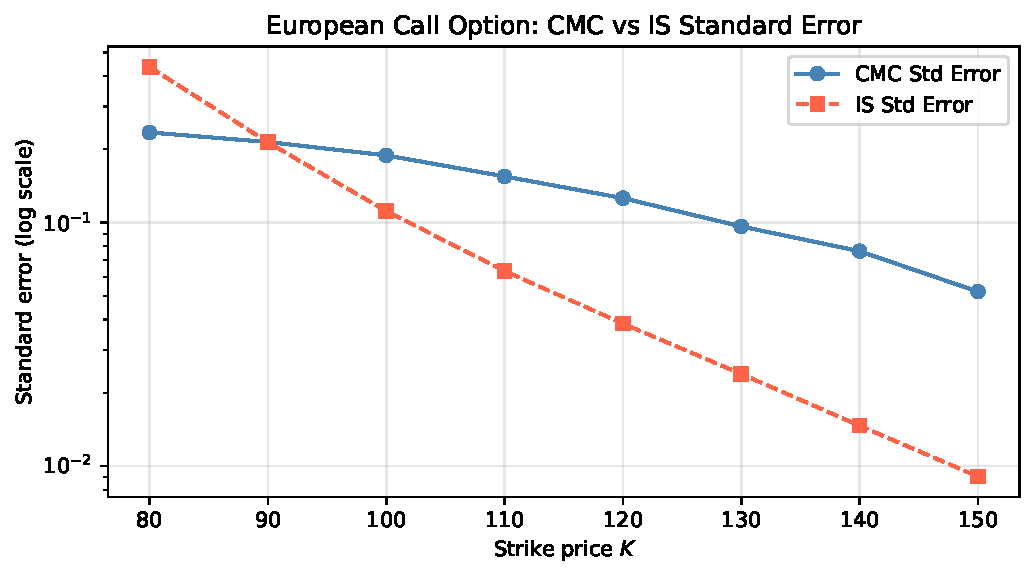
\includegraphics[width=0.72\textwidth]{fig_european_option_IS}
  \end{center}
  \small
  IS achieves substantially lower standard error for deep out-of-the-money
  options (large $K$), where CMC fails because the event is rare.
\end{frame}

% ==============================================================================
\section{5.3 Bibliographical Notes}
% ==============================================================================

\begin{frame}{5.3 Bibliographical Notes}

  \textbf{Key references:}
  \begin{itemize}
    \item \textbf{Stratified sampling and variance reduction fundamentals:}
          Rubinstein \& Kroese [186]; Asmussen \& Glynn [8]
    \item \textbf{Cross-entropy method:}
          Rubinstein [184] (original); Rubinstein \& Kroese [186] (comprehensive)
    \item \textbf{Practical tutorial on CE:} de Boer [31]
    \item \textbf{Brownian motion bisection method:}
          Asmussen \& Glynn [8]; Knuth [106]
    \item \textbf{Variance reduction for quantile/VaR estimation:}
          Chu \& Nakayama [25], Dong \& Nakayama [39], Asmussen [6]
    \item \textbf{Finance:} Black \& Scholes (1973); Hull [96]
  \end{itemize}

\end{frame}

% ==============================================================================
\section{5.4 Exercises (selected)}
% ==============================================================================

\begin{frame}[allowframebreaks]{5.4 Selected Exercises}

  \textbf{Exercise 5.T.1 (Stratified Sampling)}
  Suppose we estimate $I = \mathbb{E}Y$ with strata $A^1, \ldots, A^m$,
  $p_j = \mathbb{P}(Y \in A^j)$, cost per replication in stratum $j$ is $t_j$.
  Total budget $C$.
  \begin{enumerate}[(a)]
    \item Show $\sqrt{C}(\hat{Y}_C^{\mathrm{str}} - I) \xrightarrow{\mathcal{D}} \mathcal{N}(0, \zeta^2)$
          where $\zeta^2 = \sum_{j=1}^m \frac{p_j^2\sigma_j^2}{\gamma_j}\sum_{k=1}^m t_k\gamma_k$.
    \item Optimal allocation: $R_j \propto p_j\sigma_j / \sqrt{t_j}$.
  \end{enumerate}

  \medskip
  \textbf{Exercise 5.T.8 (Optimal IS Distribution)}
  Show that $g^*(x) = k(x)f(x)/I$ is the solution to a variational problem:
  $\arg\min_g \mathrm{Var}_g(k(X)f(X)/g(X))$.

  \medskip
  \textbf{Exercise 5.T.25 (CE Optimal Parameter)}
  For $I = \mathbb{P}(X > \gamma)$, $X \sim \mathcal{N}(0,1)$, show that the
  CE-optimal mean parameter for $\{\mathcal{N}(\theta, 1)\}$ family is:
  \[
    \theta^* = \frac{\sqrt{2}e^{-\gamma^2/2}}{\sqrt{\pi}(1 - \mathrm{erf}(\gamma/\sqrt{2}))}
  \]

\end{frame}

% ──────────────────────────────────────────────────────────────────────────────
% Summary slide
% ──────────────────────────────────────────────────────────────────────────────

\begin{frame}{Chapter 5 Summary}

  \begin{block}{Core Message}
    All variance reduction techniques aim to reduce $\mathrm{Var}(Y)$,
    equivalent to obtaining more information per simulation run.
  \end{block}

  \medskip
  \begin{tabular}{lll}
    \toprule
    Method & Key idea & When to use \\
    \midrule
    Stratified & Partition input space & Known input structure \\
    Antithetic & Negative correlation pairs & Monotone functions \\
    CRN & Shared randomness & Comparing two systems \\
    Control variates & Regression correction & Correlated auxiliary known \\
    Conditional MC & Rao-Blackwell & Can compute conditional expectation \\
    Importance sampling & Change of measure & Heavy tails / rare events \\
    Cross-entropy & Adaptive IS & Choose optimal IS distribution \\
    \bottomrule
  \end{tabular}

  \medskip
  \textbf{Finance applications:}
  Stratification + CV + antithetics + IS can each reduce variance by
  orders of magnitude for option pricing.

\end{frame}

\end{document}
